%Do not change 
\documentclass[12pt, oneside]{article}
\usepackage{amssymb,amsmath}
\usepackage[margin=1in]{geometry}
\usepackage{textpos}
\usepackage{amsthm}
\usepackage{amsfonts}
\usepackage{graphicx}

% You may add the packages you need here



\begin{document}
%Do not modify
\begin{textblock*}{4cm}(-1.7cm,-2.3cm)
\noindent {\scriptsize GEOS 254 Winter 2016} 
\end{textblock*}

%Do not modify other than putting your name where stated
\begin{textblock*}{8cm}(12.5cm,-2.3cm)
\noindent {Name: Jaime Arana-Rochel} 
\end{textblock*}


\vspace{1cm}

\makeatletter
\setlength{\@fptop}{0pt}
\makeatother

%Do not modify other than typing the homework number after #
\begin{center}
\textbf{\Large Homework \#6}
\end{center}


%Rest should contain your solution for the homework. Feel free to improvise in ways that you believe make grading easier.
\subsection*{1) Initial Value Problem}
Using Euler's Method, the estimate for $x(5)=8163403.99517$. If I use the second derivative in the calculation, $x(5)=85680022.26388$. Adding higher order derivatives, with the same stepsize, to the calculation increases the accuracy of the estimate. The estimate for $x(5)$ is higher with the second derivative because we are now including more information that we were before omitting.


\subsection*{2) Predator-Prey Model}
When $\alpha=0$, that means that there are basically no encounters between rabbits and foxes. So the equation for change in population for rabbits is simply $2R$, meaning that their population grows indefinitely since it's assumed the rabbits have an unlimited food supply and aren't being eaten. The fox equation becomes $-F$, meaning that their populations decrease as time goes one because they aren't encountering rabbits to consume.\\
As $\alpha$ increases, we see the populations of rabbits start to decrease over shorter and shorter time periods and then increase in a short time in cycles. The fox populations also cycle in shorter periods of time.\\\\
For the numerical integration of these functions, I use a step size of 0.1 to give a sufficiently smooth curve with out plotting an extremely large set of points given a smaller step size.\\
In figure 1, we that when the fox population is 200 and the rabbit population is 10, the fox population starts decreasing immediately. It isn't until the fox population is near zero when the rabbit population starts increasing rapidly. But with this rapid increase in rabbits, so does the fox density increase. This leads to a sharp decline in rabbits with the same pattern of fox population decrease seen in the beginning. This occurs in cycles.\\
In figure 2, when we've switched the starting rabbit and fox populations, it's the rabbit population which sharply decreases first since there's an abundance of food for the foxes. After the drop in rabbits, we see the same decline in foxes, but the resurgence of rabbits occurs in a shorter time frame than the last example (the cycles occur more frequently). Also noteworthy is that the rabbit population's peak numbers are always slightly more than 200, as opposed to the first example when the rabbit peak numbers were around 700.\\
For figure 3 and 4, I wanted to see what would happen if the starting populations were the same. Figure 3 shows a very similar patterns to what was observed before, but when I changed the "encounter outcome" parameter to $\alpha=0.005$, I noticed something interesting. For one, both population densities reached higher peaks than any past examples. Because the encounters were less frequent, we also see that the population drops and increases aren't as sharp as the others.\\
The last thing I tested was for different step sizes in figures 5 and 6. As expected, a step size of 1 produced a very jagged predator-prey model with a misleading plot showing cycles with a decline in peak populations growths over time. The only thing a smaller step size did was smooth out the curve for the plot. Using the same parameters as figure 2, the plots basically show the same thing.
\begin{figure}
\centering
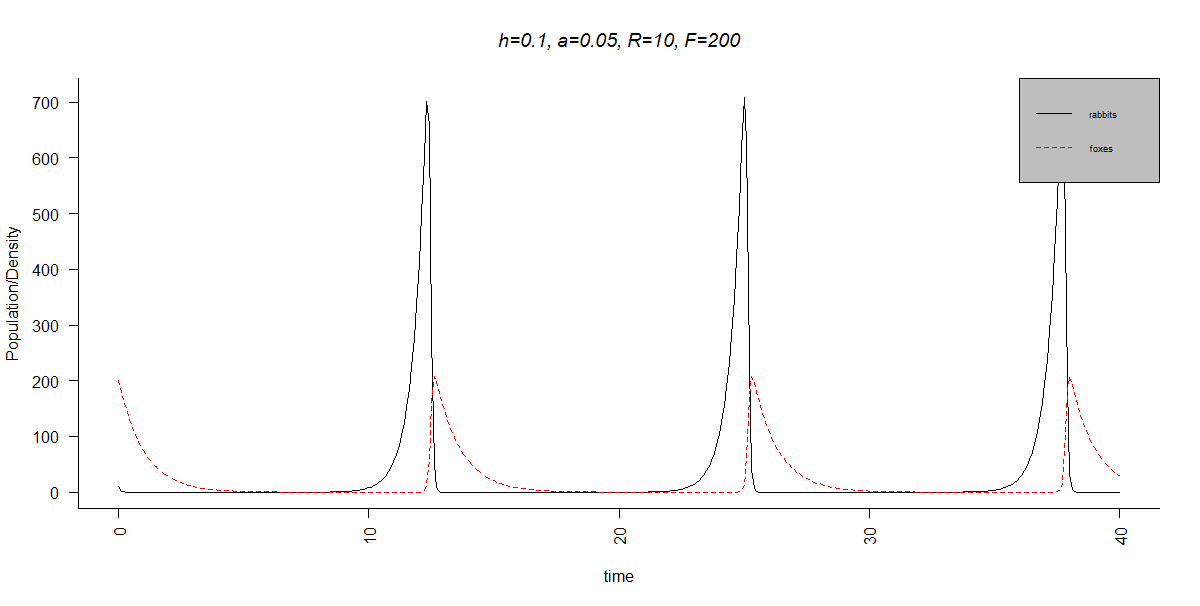
\includegraphics[width=1.1\linewidth]{./plot1}
\caption{R=10,F=200}
\label{fig:plot1}
\end{figure}
\begin{figure}
\centering
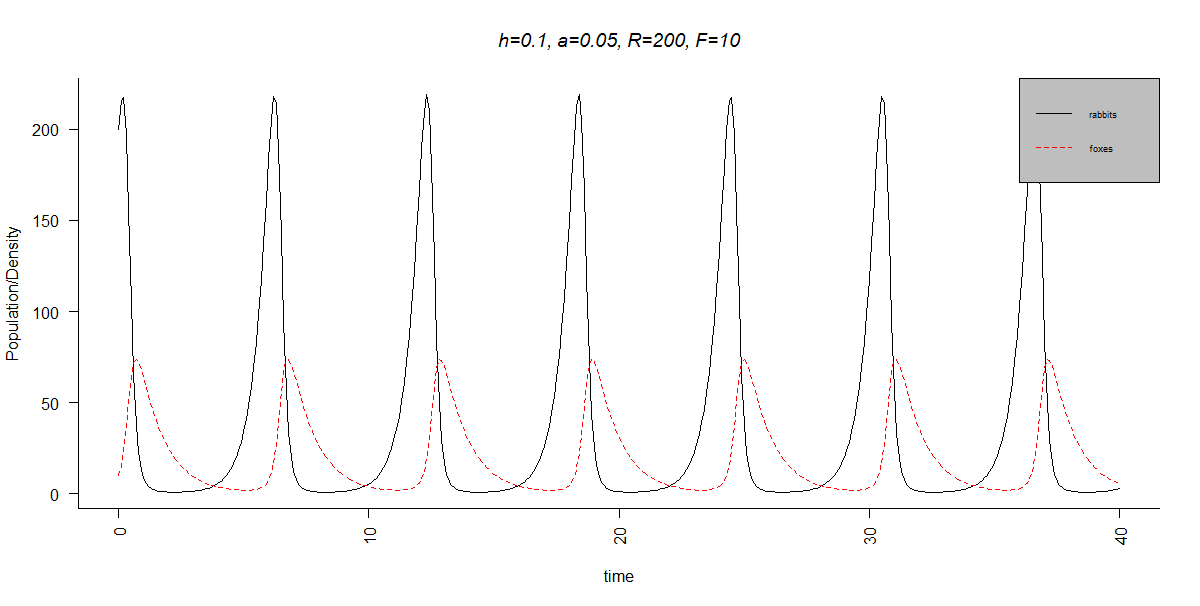
\includegraphics[width=1.1\linewidth]{./plot2}
\caption{R=200, F=10}
\label{fig:plot2}
\end{figure}
\begin{figure}
\centering
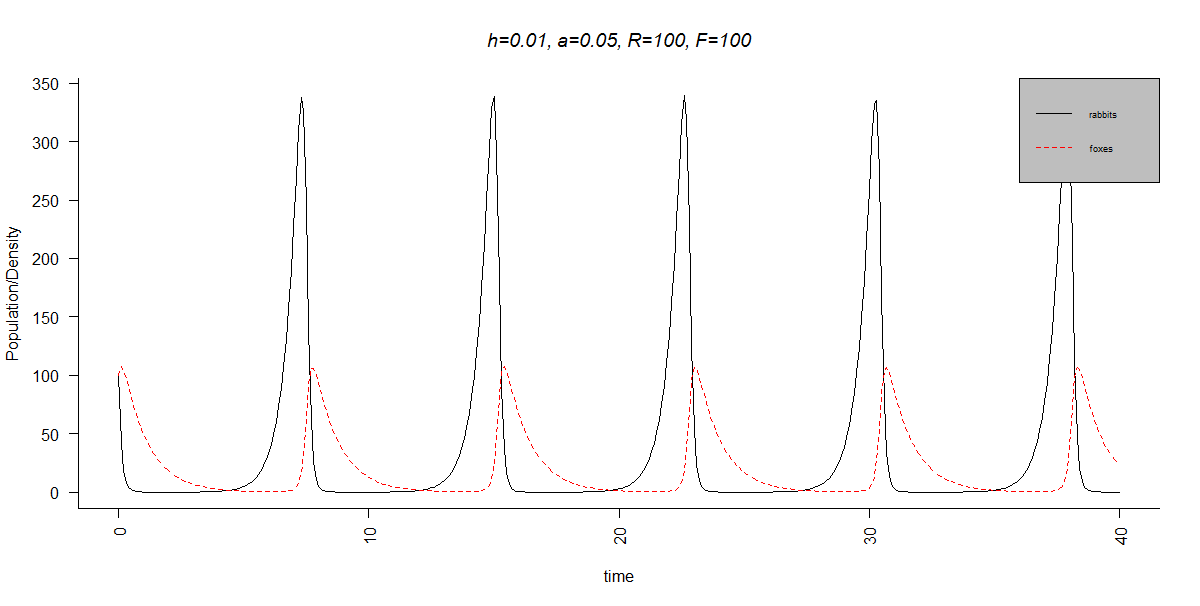
\includegraphics[width=1.1\linewidth]{./plot_r100_f100}
\caption{R=100,F=100}
\label{fig:plot_r100_f100}
\end{figure}
\begin{figure}
\centering
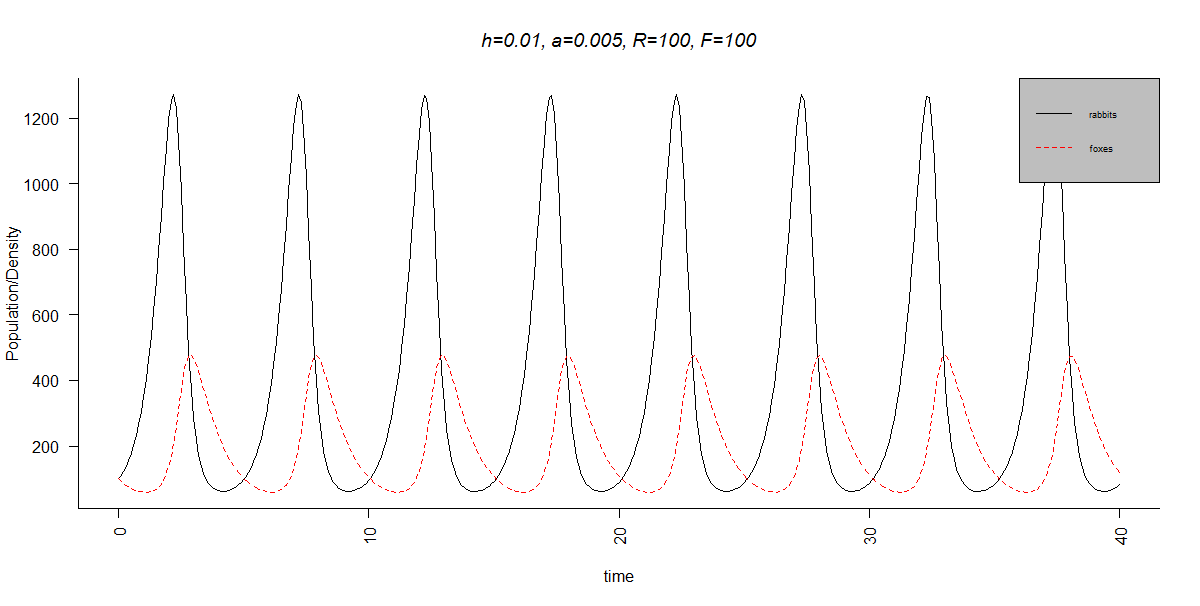
\includegraphics[width=1.1\linewidth]{./plot_a005}
\caption{R=100,F=100,a=0.005}
\label{fig:plot_a005}
\end{figure}
\begin{figure}
\centering
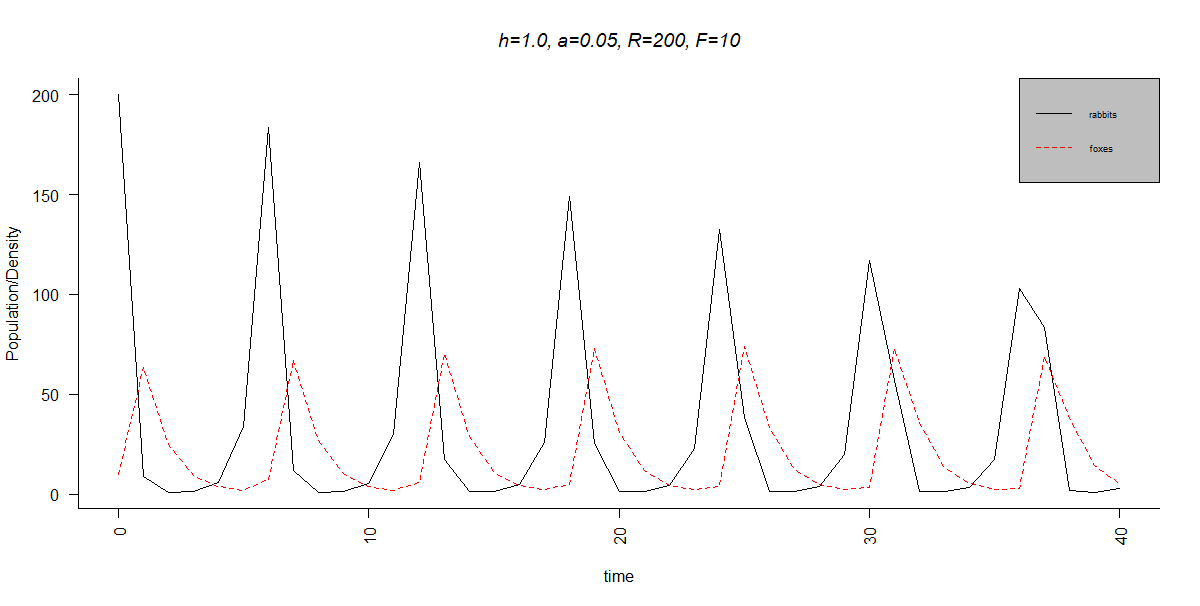
\includegraphics[width=1.1\linewidth]{./plot_step1}
\caption{h=1.0}
\label{fig:plot_step1}
\end{figure}
\begin{figure}
\centering
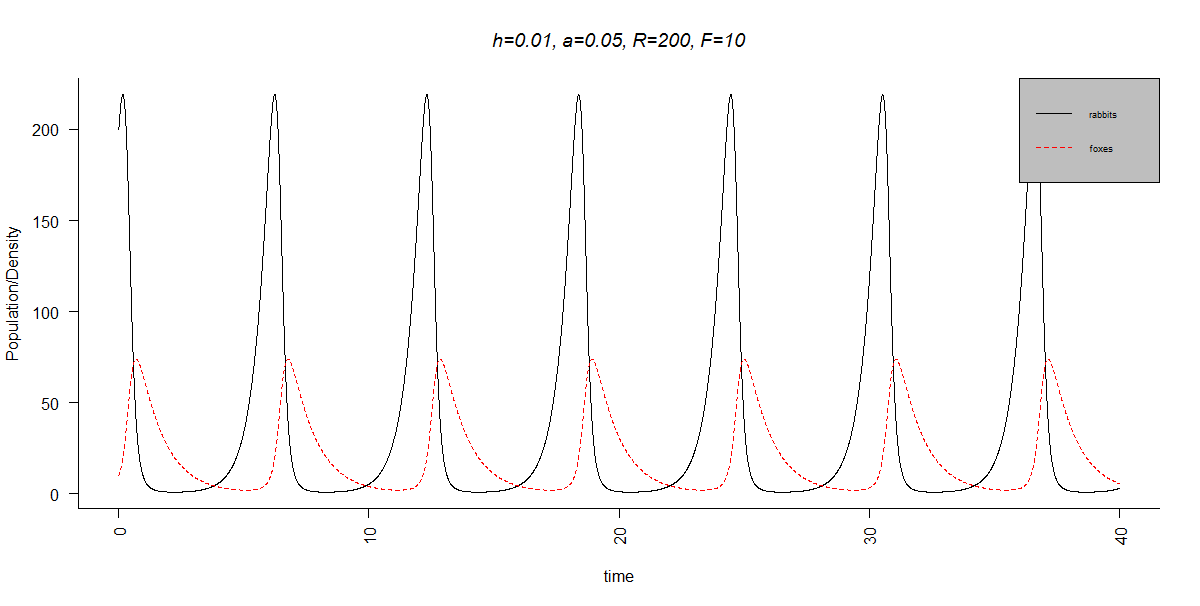
\includegraphics[width=1.1\linewidth]{./plot_step01}
\caption{h=0.01}
\label{fig:plot_step01}
\end{figure}


















\end{document}